\section{Modeling}\label{sec:modeling}
\subsection{IDP}
We assume some familiarity with the IDP system.
An extensive introduction can be found in~\cite{}.
\subsubsection{Existential Second Order}
The IDP language can express problems that consist of a set of symbols, called the vocabulary $V$, and a theory, called $T$, that uses symbols from this vocabulary.
The symbols in the vocabulary can be propositions, but they can also represent predicates and functions.
These last two types of symbols make the vocabulary, in general, a \emph{second order} object: it is an object that itself \emph{contains} not only propositional symbols, but also first order symbols.
For example, vocabulary V in Listing \ref{lst:vocabularyExample} is a second order vocabulary as it contains the first order symbol \lstinline{Edge/2}.

The theory $T$ is restricted to a \emph{first order} theory, extended with types, arithmetic, aggregates, and inductive definitions.
An example of such a theory is given in Listing \ref{lst:vocabularyExample}.
It contains an inductive definition for \lstinline{Path/2}, and one constraint.

Our inference of choice in the graph mining problem is model expansion; we search for an interpretation $I$ of symbols in the vocabulary $V$, called a \emph{model}, such that this interpretation $I$ satisfies the theory $T$.
This corresponds to the implicit \emph{existential quantification} of all symbols in the vocabulary, both the propositional as well as the first order symbols.
In the example of Listing~\ref{lst:vocabularyExample}, we expand the $S$ to the model $Result$ with 3 edges: One from the first node to itself, one from the first node to the second, and one from the second to the third.
Path contains all corresponding paths between these three nodes.

In conclusion, we say IDP can express model expansion for \emph{Existential Second Order} problems.
This level of expressiveness is not sufficient for general graph mining problems.
We will discuss the several issues in the remainder of this section.

\lstset{basicstyle=\scriptsize\ttfamily,breaklines=true}
\begin{lstlisting}[mathescape,style=model,caption=\ldots, label=lst:vocabularyExample]
vocabulary V{
    type Node
    Edge(Node, Node)
    Path(Node, Node)
}
theory T : V {
    $\forall$n[Node] : $\exists$n2[Node] : Edge(n,n2) $\lor$ Edge(n2,n).
    {
        Path(x,y) $\leftarrow$ Edge(x,y).
        Path(x,y) $\leftarrow \exists$z[Node] : Path(x,z) $\land$ Path(z,y).
        Path(x,y) $\leftarrow$ Path(y,z).
    }
}
structure S : V{
    Node = {1;2;3}
}

structure Result:V{
    Node = {1; 2; 3}
    Edge = {1,1; 1,2; 2,3}
    Path = {1,1; 1,2; 1,3; 2,1; 2,2; 2,3; 3,1; 3,2; 3,3 }
}
\end{lstlisting}


%problems in which there is an existentially quantified, generally second order, vocabulary of symbols and a first order theory with symbols from that vocabulary.
\paragraph{Issue 1}
First, we must represent the set of example graphs, as specified in \textbf{Def.}~\ref{def:gm2}. 
This definition uses a higher order predicate(See \textbf{Listing}~\ref{lst:HOPred}) \lstinline{GraphInst/3} with as first argument the edge predicate and as second argument the label function. For the first graph, \lstinline|{1,2; 2,1}| and \lstinline|{1\mapsto a; 2\mapsto b}| respectively. 
It represents a single graph as a tuple of predicates and functions, visualized in \textbf{fig.}~\ref{fig:LocalCoherence} as the solid shape.
It is clear that this representation is highly locally coherent, and preserves the independence of graph characteristics.
However, as we are restricted to \emph{Existential} Second Order, we cannot express this higher order predicate in IDP.

One possible solution is to replicate for each graph the different characteristic predicates and functions, as shown
in \textbf{Listing}~\ref{lst:multiglobal} and visualised as the dashed shapes in \textbf{Fig.}~\ref{fig:LocalCoherence}.
In this encoding, every graph has its own edge predicate and label function. 
Because there is now no relation between the different edge predicates and label functions, it is necessary to formulate our theory in terms of these different predicates and functions.
Encoding a property such as ``In every graph, all nodes have at least two \matthias{outgoing} edges'' must be stated for each of the edge predicates explicitly:
%duplicate in our theory the constraints and properties (i.e. homomorphism) about these example graphs and their relations as well: we cannot generalize over the names of these edge relations and labeling functions.
\begin{center}
\begin{tabular}{c}
\begin{lstlisting}[mathescape]
$\forall$ n[Node] : $\exists$ n1,n2[Node] : E1(n, n1) $\land$ E1(n,n2) $\land$ n1 $\neq$ n2.
$\forall$ n[Node] : $\exists$ n1,n2[Node] : E2(n, n1) $\land$ E2(n,n2) $\land$ n1 $\neq$ n2.
\end{lstlisting}
\end{tabular}
\end{center}

It is clear that this solution is undesirable due to the way it scales and the theory modifications needed with growing problem instances.
It retains the local coherence and independence of graph characteristics when it comes to data representation, but prohibits the abstraction (generalization) of knowledge in the theory.
% about these properties, as evidenced by our obligation to duplicate the theory for each graph.

%GraphInst(E:Node$\times$Node,Lb
\begin{lstlisting}[mathescape,caption=Higher order predicate modeling the set $\graphset{G}$ of Def~\ref{def:gm2}.,label=lst:HOPred]
GraphInst({1,2; 2,1},{1$\mapsto$a; 2$\mapsto$b},pos).
GraphInst({1,3; 2,1},{1$\mapsto$c; 2$\mapsto$b; 3$\mapsto$a},neg).
\end{lstlisting}
\begin{minipage}[t]{0.45\linewidth}
\begin{lstlisting}[mathescape,caption=Multiple individual global relations,label=lst:multiglobal]
E1(1,2). lb1(1)=a.
E1(2,1). lb1(2)=b.
E2(1,3). lb2(1)=c.
E2(2,1). lb2(2)=b.
         lb2(3)=a.
\end{lstlisting}
\end{minipage}
\begin{minipage}[t]{0.1\linewidth}
 ~
\end{minipage}
\begin{minipage}[t]{0.45\linewidth}
\begin{lstlisting}[mathescape,caption=Disjoint union using indexed global relations,label=lst:indexedglobal]
E(g1,1,2). lb(g1,1)=a.
E(g1,2,1). lb(g1,2)=b.
E(g2,1,3). lb(g2,1)=c.
E(g2,2,1). lb(g2,2)=b.
           lb(g2,3)=a.
\end{lstlisting}
\end{minipage}




A more workable solution is to represent each characteristic property, such as the edge relation, by a single global relation for all graphs, as shown in \textbf{Listing}~\ref{lst:indexedglobal} and by the dotted shape in \textbf{Fig.}~\ref{fig:LocalCoherence}.
This relation behaves the way it should for a specific graph instance based on an additional argument serving as an identifier for the graph of interest.
%This gives rise to a set $G$ of \emph{graph identifiers}, one for each example graph.
This global relation now corresponds to the \emph{disjoint} or \emph{tagged union} of the graphs' relations, where the tags are drawn from a set $G$ consisting of graph identifiers.
It is clear that this representation forces us to give up the local coherence of graph characteristics that was present in \textbf{Def.}~\ref{def:gm2}.
%Nu kunnen we kijken wat deze truuk doet met onze mogelijkheid om de abstraction van de theory uit te drukken. Normaal mwillen we dit zo schrijven. Hoewel we nu de generalisatie kunnen uitdrukken, verplicht de restrictie tot existentieel s..o ons om de homomorphic mapping functies te tot een globale property te promoveren, hoewel we feitelijk niet geinteresseerd zijn in de concrete mappings. om om te gaan met de afhankelijkheid van deze functies op de spec. vb grafen moeten we... die nu erg lijkt op skolemisation. theory

%Using this trick however, does not influence our ability to 
Now we can generalize over the different graphs, so that we can encode the property stated above as:
\begin{lstlisting}[mathescape]
$\forall$ gid[GraphId] : $\forall$ n[Node] : $\exists$ n1,n2[Node] : E(gid, n, n1) $\land$ E(gid, n,n2) $\land$ n1 $\neq$ n2.
\end{lstlisting}
%But can we now express the abstraction (generalization) of knowledge about these properties, such as the positive homomorphic property?
%to separate the constraint describing the positive homomorphic property, and the coint on its number of occurrences.
%This, from a KR point of view, 
%Furthermore, the restriction to ESO requires us 
%As an example, we illustrate this trick by showing on the expression of the positive homomorphic property, where it greatly resembles Skolemization.
%As evidenced in \textbf{Def.}~\ref{def:gm2}, normally one would express the positive homomorphic property by quantifying (counting) over all graphs, requiring the existence of a function with the correct properties.
%Using the disjoint union representation, we can quantify over the set $G$ of graph identifiers instead of over the actual graphs.
%Therefore, this representation allows us to express this property.

\begin{figure}[h]
\centering
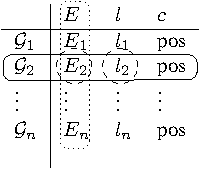
\includegraphics{CoherenceTable-crop.pdf}
\caption{Local coherence\label{fig:LocalCoherence}}
\end{figure}

%These three different ways of representing graphs are summarized in Fig~\ref{fig:LocalCoherence}.

\paragraph{Issue 2}
%Having solved\matthias{circumvented?} our first issue, 
Next, we would like to express the homomorphic property.
This can be done using a count aggregate, as shown in Listing~\ref{lst:QuantifyOutsideVocabulary}.
First we express the set of all example graphs to whom there exists a homomorphism from our pattern.
% generate the set of all example graphs to whom we can find a homomorphism from our pattern.
We do this by quantifying over all example graphs g or, per \textbf{issue 1}, their identifiers, and subsequently 
expressing the condition under which they are part of this set: i.e. that there must exist a function f that represents a homomorphism from our pattern graph $p$ to $g$.
In principle, we could then proceed by counting the number of elements in this set.

\begin{lstlisting}[mathescape, caption=Quantifying over functions outside the vocabulary, label=lst:QuantifyOutsideVocabulary,basicstyle=\fontfamily{lmvtt}\selectfont]
#{$\forall g \mid g \in G \land \exists$ $f$ : $f$ is a homomorphism from $p$ to $g$ }
\end{lstlisting}
However, working in IDP, the restriction to ESO forbids us to quantify over first-order entities such as the functions f from \textbf{Listing}~\ref{lst:QuantifyOutsideVocabulary} outside of the vocabulary.
Thus, we are required to promote the homomorphic mapping functions to a global property in the vocabulary, even though we are only interested in the existence of a mapping, and not in a concrete valid mapping itself.
We prevent the same explosion of mapping functions as with the graph characteristics above, using the same method as above. Note that in this case, it corresponds to Skolemization.
We introduce a general function \verb|f| that represents all homomorphisms, and make its dependency on a specific example graph explicit using an additional argument:
\verb|partial f(graphId, node):node|.
%As it is impossible
%We introduce a general function \verb|f| that represents the homomorphisms, and make its dependency on a specific goal graph explicit using an additional argument:
In Second Order Logic, this dependency would follow directly from the order of the separate quantifications.

We can now use this \verb|partial f| anywhere we would use the regular homomorphic function for a specific graph by fixing the chosen example graph.
Note that this encoding also requires us to make this function \verb|f| partial, as the Graph Mining problem does not require the solution to be homomorphic with \emph{all} example graphs.
%\todo{Of course, other (even uglier) schemes exist to encode this. Should we mention this?}


\paragraph{Issue 3} Much in the same way, limiting ourselves to existential second order prohibits us from expressing the negative homomorphic property (the pattern is homomorphic with no more than $N_{-}$ negative examples) in the same model.
In fact, the negative homomorphic constraint asserts a property for all candidate homomorphic functions, which would lead to \emph{universal} quantification.
Therefore, our only recourse is to encode its dual positive constraint and require it to fail when queried.

Take, for example, the template, pattern candidate and positive and negative example graphs from \textbf{Fig.}~\ref{fig:ex2}.
Assume all nodes have the same label.
With parameters $N_{+}=1$ and $N_{-}=0$, this pattern candidate is clearly an invalid pattern: It is homomorphic with both the positive and the negative example.
Suppose we express the negative homomorphic property directly, changing only the comparison operator used on the count aggregate from $\geq$ to $\leq$.
Because we now look for one general (Skolemized) homomorphic function, we can choose a single global function which represents a homomorphism with the positive example graph, but not with the negative example graph.
An example of such a solution is shown in Listing~\ref{lst:invalidf}.

If we want to prevent these invalid models, we must encode the dual positive constraint, and require it to fail. 
However, to do this in IDP, we need another theory and provide procedural (lua) code that ties these theories and their inferences together. 
It must pass models from the theory that asserts the positive property to the theory that checks the negative property. This procedural code is clearly not declarative.
In much the same way, IDP cannot express the isomorphism restriction when looking for multiple patterns: if needed, this restriction is transformed into a dual positive restriction (there \emph{must} be an isomorphism) and is required to fail as well. These two theories expressing the dual of the negative homomorphism property and that of the isomorphism restriction can safely be merged.


\textbf{ASP}, a language family closely related to IDP, can prevent the invalid models of the example above by leveraging the minimality property of their models: ASP looks for the minimal answer set models, whereas idp looks for well-founded models.
This technique is called the \emph{saturation} technique~\ref{eiter} and can prevent the procedural code that IDP requires.

When using this technique, ASP detects negative example graphs for which the f does not represent a homomorphism, and 
requires for these example graphs that $f$ must map every node of the pattern on every node of that example graph, dropping the injectivity constraint.
This way, $f$ becomes so large that it is impossible that it belongs to the minimal answer set unless there is no homomorphism from the pattern to this (negative) example graph.
Consequently, the minimality property will cause the solver to look for an $f$ that represents a homomorphism for as many example graphs (including negatives) as possible.
The same technique can be applied to the isomorphism restriction.
 %requiring that in this case f must be the total relation
%accordingly enlarging the answer set by requiring that in these cases f must be the \emph{total} relation for this graph, the minimality property will cause the solver to look for $f$ that represent a homomorphism for as many example graphs (including negatives) as possible.


While this technique succesfully prevents the need of a procedural loop and the rewriting of the negative homomorphic property and the isomorphism restriction, it is clear that this technique is not derived from a natural KR translation of the Graph Mining definition.
\matthias{Also, it forces to look for homomorphisms for every negative example graph, whereas $N_{-}$ + 1 example graphs are enough. Quite possible that there is a workaround for this however.}
\begin{figure}
  \centering
  \begin{subfigure}[b]{0.15\textwidth}
    \centering
    \begin{tikzpicture}[scale=.5]
      \node[vertex] (a) at (1,1) {};
      \node[vertex] (b) at (2,1) {};
      \node[vertex] (c) at (2.7,2) {};
      \node[vertex] (d) at (2,3) {};
      \node[vertex] (e) at (1,3) {};
      \node[vertex] (f) at (0.3,2) {};
      
      \draw (1,1) -- (2,1) -- (2.7,2) -- (2,3) -- (1,3) -- (0.3,2) -- (1,1);
      \draw (1,1) -- (2,3);
      \draw (2.7,2) -- (0.3,2);
      \draw (1,3) -- (2,1);
    \end{tikzpicture}
    \caption{Template}
  \end{subfigure}
  ~
  \begin{subfigure}[b]{0.22\textwidth}
    \centering
    \begin{tikzpicture}[scale=.5]
      \node[vertex] (a) at (1,1) {};
      \node[vertex] (b) at (2,1) {};
      \node[vertex] (c) at (2.7,2) {};
      \node[vertex] (d) at (2,3) {};
      \node[vertex] (e) at (1,3) {};
      \node[vertex] (f) at (0.3,2) {};
      
      \node[circle] at (1,0.7) {a};
      \node[circle] at (2,0.7) {b};
      \node[circle] at (3,2) {c};
      \node[circle] at (1.6,3.8) {g1};
      \draw (1,1) -- (2,1) -- (2.7,2) -- (2,3) -- (1,3) -- (0.3,2) -- cycle;
      \draw (1,1) -- (2,3);
      \draw (2.7,2) -- (0.3,2);
    \end{tikzpicture}
    \caption{Positive Example}
  \end{subfigure}
  ~
  \begin{subfigure}[b]{0.23\textwidth}
    \centering
    \begin{tikzpicture}[scale=.5]
      \node[vertex] at (0,0) {};
      \node[vertex] at (1,1) {};
      \node[vertex] at (2,0) {};
      \node[vertex] at (3,1) {};
    
      \node[] at (0,-0.2) {d};
      \node[] at (1,1.2) {e};
      \node[] at (2,-0.2) {f};
      \node[] at (3,1.2) {g};
      \node[] at (1.6, 2.8) {g2};
      \coordinate (1) at (0,0);
      \coordinate (2) at (1,1);
      \coordinate (3) at (2,0);
      \coordinate (4) at (3,1);
      \draw (1) -- (2) -- (3) -- (4);
    \end{tikzpicture}
    \caption{Negative Example}
  \end{subfigure}
  ~
  \begin{subfigure}[b]{0.22\textwidth}
      \centering
      \begin{tikzpicture}[scale=.5]
        \node[vertex] at (1,2) {};
        \node[vertex] at (2,3) {};
        \node[vertex] at (3,3) {};
        
        \node[circle] at (0.9,2) {1};
        \node[circle] at (2,3.3) {2};
        \node[circle] at (3.15,3.3) {3};
        \draw (1,2) -- (2,3) -- (3,3);
      \end{tikzpicture}
      \caption{Pattern Candidate}
  \end{subfigure}
  \caption{Example 2\label{fig:ex2}}
\end{figure}

\begin{minipage}{\linewidth}
\begin{lstlisting}[mathescape,caption=An possible assignment for f, label=lst:invalidf]
f={
    g1,1$\mapsto$a, g1,2$\mapsto$b,g1,3$\mapsto$c,
    g2,1$\mapsto$d, g2,2$\mapsto$e,g2,3$\mapsto$g
}
\end{lstlisting}
\end{minipage}

%\matthias{Find a convincing but small example}
%\matthias{The moment to introduce the asp saturation technique}

%\paragraph{ASP}
%Let us describe a way to encode the problem into ASP. Conceptually we need to handle three constraints: matching of positive examples, not matching of negative examples and canonicity (that only not isomorphic graphs are produced).

\subsubsection{Inductive Definitions}
Beyond the Existential Second Order restriction, the IDP language is also extended with inductive definitions. These definitions, evaluated under the well-founded semantics, allows the derivation of negative knowledge that otherwise would be underivable.
For example, in \textbf{Fig.}~\ref{fig:trans}, without using inductive definitions, one is unable to derive that point $a$ and $b$ are not connected.
\begin{figure}[h]
    \centering
   \begin{tikzpicture}[scale=0.7]
       \node[vertex] at (1,1) {};
       \node[vertex] at (2.2,1) {};
       \node[vertex] at (2.7,2) {};
       \node[vertex] at (1,1.3) {};
       \node[vertex] at (1.8,2.3) {};
       \node[vertex] at (2.7,2.3) {};
   
       \node[circle] at (2.2,0.7) {a};
       \node[circle] at (1.8,2.65) {b};
     
       \draw (1,1) -- (2.2,1) -- (2.7,2) -- cycle;
       \draw (1,1.3) -- (1.8,2.3) -- (2.7,2.3) -- cycle;
   \end{tikzpicture}
\end{figure}
%\reversemarginpar
%\todo{A section about inductive definitions, and their use. (Being able to derive negative knowledge)}

\subsubsection{Other inferences}
One of the advantages of IDP is its underlying \emph{Knowledge Base} paradigm~\ref{}.
Essentially, this paradigm ensures that we can perform other inferences on the graph mining problem, e.g. finding patterns with as many or as few nodes as possible, without modifying the specification.

\reversemarginpar

\subsection{ProB}
The ProB System can handle mathematical specifications using higher order logic and set theory.
As a result, ProB specifications can cover the polynomial hierarchy \textbf{PH}.

\subsubsection{Higher Order}
Because of ProB's Higher Order support, we can treat graphs as the inherent higher order objects with structure $\triple{E,l,c}$ that they are.
This allows us to quantify over a graph and easily access all its characteristic predicates and functions.

ProB's support for higher order also makes it possible to quantify over the functions $f$ that represent homorphisms locally: there is no need to declare the function f globally, instead they are defined within the context of the set of homomorphic positive (negative) examples.
Here, the representation of these functions $f$ is direct, without graph identifier that corresponds to the disjoint union technique as proposed for IDP.
Instead, the graph \graph{G} for which a homomorphic function is sought, is brought in scope by the quantifier of the set expression.

Because these are now quantified locally, the solver will find a homorphism if one exists, regardless of whether we are expressing the positive or negative homomorphism property.
As a result, ProB can model the negative homomorphism property directly, without the need for a second theory and procedural tie-in code.

The same reasoning allows ProB to model the isomorphism restriction when looking for multiple patterns.
\subsubsection{Inductive definitions}
ProB cannot natively handle inductive definitions.
This makes it difficult to model the connectedness requirement of patterns.
Recently, efforts have been made to integrate Kodkod, which provides a high-level interface to SAT-solvers~\citep{DBLP:conf/tacas/TorlakJ07}, into ProB~\citep{DBLP:conf/fm/PlaggeL12}.
\matthias{How does the translation and mapping mechanism of ProB $\leftrightarrow$ KodKod compare to our ideas of oracles?}


\subsection{Conclusion}

%\section{Feature Comparison}
%
%\subsection{IDP} 
%
%\textbf{Pro:}
%\begin{itemize}
%  \item can model inductive definitions
%  \item allows core formulation in a high-level language (NP)
%  \item handles aggregates
%  \item has support for variety of constraints
%\end{itemize}
%\textbf{Cons:}
%\begin{itemize}
%  \item cannot handle negative case $\textit{NP}^\textit{NP}$ complexity
%  \item cannot model subgraph isomorphism independence
%  \item cannot handle dominance, i.e., when one model is preferred over another 
%\end{itemize}

\matthias{This table~\ref{tbl:conclusion} is not in the correct place yet. It is an early draft, and must be cleaned up and introduced properly}
\def\checkmark{\tikz\fill[scale=0.4](0,.35) -- (.25,0) -- (1,.7) -- (.25,.15) -- cycle;} 

\begin{table}[h]
\begin{center}
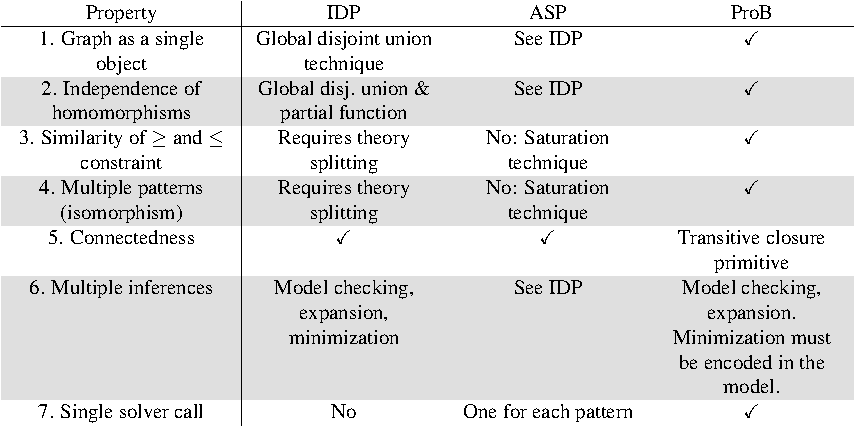
\includegraphics{PropertyTable-crop.pdf}
\end{center}
\caption{Evaluation of the desirable properties in IDP / ASP / ProB\label{tbl:conclusion}}
\end{table}

